\documentclass[a4paper]{article}
\makeatletter
\newcommand*{\rom}[1]{\expandafter\@slowromancap\romannumeral #1@}
\makeatother
\usepackage{hyperref} %для гипперссылок
\usepackage{setspace} %межстрочный интервал
\usepackage{ragged2e} %выравнивание
\usepackage{fancyhdr} %заголовки
\usepackage{titlesec} %опять заголовки шрифты размеры тыры пыры
\usepackage{setspace} %временное изменение межстрочного интервала
\usepackage{newtxtext, newtxmath} %для таймс ню роман
\usepackage{microtype} %для лучшего типографического оформления
\usepackage{multicol} %для колонок
\usepackage[utf8]{inputenc} %для специальных символов
\usepackage{enumitem} %для списков
\usepackage{hyphenat} %для переносов
\usepackage{graphicx} %для картинок
\usepackage{wrapfig} %обтекание картинок
\usepackage{float} %ещё штука для картинок 
\usepackage[left=2.2cm,right=2.2cm, top=1.5cm,bottom=2cm]{geometry}
\newcounter{mycounter}
\setlist[itemize]{noitemsep, topsep=0pt} % убрать отступы itemize
\fancyhf{} % очищает все верхние и нижние колонтитулы.
\cfoot{\textbf{\thepage}} % жирные номера страниц
\pagestyle{fancy}
\setcounter{page}{171} % настройка нумерации страниц
\setlength{\columnsep}{.5cm} % интервал между колонками
\renewcommand{\headrulewidth}{0pt} %убирает сомнительную линию

\linespread{1.0} %межстрочный интервал

\setlength{\columnsep}{0.5cm} %расстояние между колонками

\begin{document}

\setlength\parindent{11pt}
\fontsize{10}{13}\selectfont

\title{
 \begin{spacing}{0.7} %местное уменьшение интервала  
  {\Huge\nohyphens{Applied Aspects of Using OSTIS Technology in
Information Support of Digitalisation of Water
Use Processes of Dairy Processing Enterprises}}
 \end{spacing}
}
\author{ 
 \linespread{1.3} Vladimir N. Shtepa\\Minsk, Belarus\\Email: tppoless@gmail.com                  %увеличение межстрочного интервала на 30%
 \and
 Eduard N. Muslimov\\Minsk, Belarus\\Email: muslimoven@mail.ru
}
\date{}
\maketitle
\begin{multicols}{2}
\normalsize{\begin{spacing}{0.1}

{\textbf{ %жирный текст
\fontsize{10}{19}\selectfont
\textit{Abstract}—The conceptual approaches of digitalisation of
manufactures based on the e-Manufacturing ideology are
evaluated, which are proposed to be used for modelling
the processes of water use of milk processing enterprises;
the organisational and technological processes of formation
of pollutants in their wastewater are analysed. In IDEF0
methodology functional modelling of water use of such
productions is carried out, that allowed to reveal complexity
and multidirectionality of interrelations of parameters and
to justify the use of OSTIS technology for tasks of formation
of intellectual information and reference system. On the
example of a biological pond as a node of wastewater
treatment, an element of the proposed approach of practical
implementation of OSTIS-solutions in the segments of
digital modelling of the dairy industry and environmental
management is implemented.
}
\par\textbf{\textit{Keywords}—Digitalisation, water management, milk processing, information and reference system }}
\end{spacing}}
 \vskip 1cm
\begin{center}
\rom{1.} Introduction
\end{center}
 

\fontsize{10}{13}\selectfont \nohyphens{
The term Digitale Fabrik (digital factory) is used to describe production in the context of informatisation, but today the essence of Digitale Fabrik is more often expressed by the term e-Manufacturing. At the heart of the idea of e-Manufacturing is the continuous application of digital models in the design and operation of production systems. Not only the products themselves are modelled, but also production equipment, material flows, as well as production and logistics processes, taking ergonomics and human factors into account. The goal of e-Manufacturing is to achieve such a level of object and process modelling that the real manufacturing process starts only after all its elements have been studied and optimised with the help of models [1]. \par Digital manufacturing is one of the components of product lifecycle management (PLM) technology, its main task is to improve complex manufacturing processes. A set of digital manufacturing solutions belongs to the class of MRM-systems (Manufacturing Process Management) [2]. \par If in CAD/CAM/CAE-systems in most cases the application of a particular software tool is associated with obtaining a digital layout of the product and the distribution of roles is clearly deterministic by the content of the work performed (surface designer, layout designer, solid geometry designer, etc.), in MRM-systems this dependence is much more flexible [3]. This is due to the fact that technological processes in different industries can differ significantly, even enterprises of the same industry can have different technological processes. Such operations include the functioning of complexes ensuring the fulfilment of environmental requirements, including the removal (treatment, discharge) of industrial wastewater (WW) [4], [5]. \par This problem is especially acute for enterprises of milk processing industry.  \vskip 0.2cm \rom{2.} Technological problems of formation and treatment of wastewater of milk processing enterprises \vskip 0.2cm Contaminated wastewater of milk processing plants is a product formed after washing of equipment, technological piping system, transport tanks of different volumes, including road and railway tanks, flasks and other containers [6], [7]. Also the sources of pollutants formation include effluents after cleaning of production facilities, washing of panels and floors. The amount of polluted wastewater is 20\% — 50\% of the total volume of water use. Wastewaters of milk processing enterprises belong to the category of highly concentrated organic pollutants: they contain significant concentrations of organic pollutants (fat, protein, lactose), polluted also with inorganic compounds (including acids and alkalis) and synthetic surface active substances (detergents). Their composition and concentration of pollutants depend on the profile and productivity of enterprises [7], [8]. \par Analysis of literature sources [4]–[8] has shown that there is an intensive search for rational and highly efficient methods and technologies of wastewater treatment for food industry enterprises (including dairy industry). The most common solution in this area is the combination of classical treatment methods with new methods [8], while an adequate choice of equipment for a particular enterprise is impossible without a high-quality design task and the preparation of appropriate models (first of all, water technological passport), including those based on digital technologies [9].} 
\newpage \nohyphens{
\begin{center}

\rom{3.} Problem formulation for an intelligent information \par
and reference system water use by dairy processing \par
enterprises\end{center}
\vskip 0.2cm
\par To solve the problem, we initially perform functional
modelling in IDEF0 methodology (Fig. \rom{3}).\par The following categories of parameters (according
to IDEF0 terminology) are selected on the basis of
technological analysis:}
\begin{itemize}[leftmargin=7mm]

    \item \textbf{input factors}
      \begin{itemize}[leftmargin=3.5mm]
      \item coming from measuring instruments in operational mode:
        \begin{itemize}[leftmargin=5.3mm]
            \item  actual flow rate of process water (PW):;
            \item  about 2-3 process water quality indicators
(e.g., pH, electrical conductivity);
            \item actual wastewater flow rate;
\item\nohyphens{ about 3-5 quality indicators of WW: pH, temperature, redox potential (ORP), chemical oxygen demand (COD), electrical conductivity;}
\item information on equipment status (based on the
production scheme and operating SCADA).
        \end{itemize}
        \item measurements of water quality parameters from
the laboratory:
\begin{itemize}[leftmargin=5.3mm]
\item information on PW quality;
\item information on WW quality.
\end{itemize}
\item from expert technologists and expert technicians:
\begin{itemize}[leftmargin=5.3mm]
\item information on the planned demand for PW
per shift;
\item \nohyphens{information on the planned demand for ingredients per shift;}
\item information on the state of technological
equipment.
\end{itemize}
      \end{itemize}
       \item\nohyphens{ \textbf{control factors:} requirements for the quality of PW,
characteristics of the equipment (under which it
operates according to its passport parameters), requirements for technological processes (under which
the requirements for their regulatory flow are met),
regulatory requirements for the quality of wastewater, cost of resources;}
 \item\nohyphens{ \textbf{mechanisms:} electrical equipment that ensures the
operation of the information system as a whole;}
 \item \textbf{results:}
  \begin{itemize}[leftmargin=3.5mm]
      \item\nohyphens{ dynamic balance of water use (based on planned
shift production tasks, as well as with the function
of calculating financial costs for the period from
the beginning of the shift to the current point
in time - potentially a forecast is also necessary
based on the current state, for example, until the
end of the shift);}
\item\nohyphens{ operational forecast of the quality of WW (based
on planned shift tasks, as well as with a forecast
correction function based on real indicators of
production and quality of PW and WW at the
current time (with various forecast projections);}
\item\nohyphens{ dynamic recommendations for organizational,
technical and technological actions in order to
reduce financial costs for water use (based on the
current situation and forecast);}
\item\nohyphens{ dynamic costs for minimizing waste pollution
(based on the current situation and forecast).}
\end{itemize}
    \end{itemize}
   \par\nohyphens{ Performing a decomposition of the first level diagram
(see \ref{Fig. 1}) allows you to detail the tasks of digital
modeling (Fig. \rom{3}).\par
Analysis of the diagram of the first level of decomposition (see Fig. \rom{3}):}
\begin{itemize}[leftmargin=7mm]

    \item\nohyphens{ here the key will be the multi-level decomposition of
the block “Systematization of data on water disposal
parameters”, it will include production subsystems
and units that use “process water”, polluting it
and transforming it into “waste water” - with the
main module “Intelligent information and reference
system" (IIRS), which will analyze the situation
and "consult" process and technical specialists: what
operating modes they should choose initially, how
to relate to the state of this or that equipment (the
flow of production processes), what variants of the
assortment task will lead to what resource costs and
environmental risks, regarding the resource cost of a
specific assortment task, regarding the acceptability
of the functioning of a specific unit or the use of an
ingredient, etc. (based on a retrospective production
analysis);}
\item\nohyphens{ at the same time, the “Intelligent Information and
Reference System” must, of course, work with the
integrating technology support block “Analysis and
forecasting of the efficiency of use of water resources of an enterprise.”}
    \end{itemize}
    \par\nohyphens{
    The “intelligent information and reference system”, in
fact, should become an adaptive (interactive) technological regulation for water use of an enterprise, largely
ensuring the interoperability of the entire system as a
whole, with potential transformation along the chain:
“decision support system – automated process control
system for water use — digital MES (MIS, LIMS, EMI)
resources — ERP.”
\par
Then the intelligent information and reference system
for supporting specialists of milk processing enterprises
in the water use segment is a software product (SP)
intended for storage in a structured electronic form
and prompt provision to other SPs and specialists of
various technological information accumulated both in
basic regulatory documents (BC ,SS R, BAT) and in
specially created databases and knowledge. IISS will
make it possible to create a unified information space
of technological knowledge for prompt consultation on
issues of interest to specialized specialists (managers,
chief engineers, WW technologists, instrumentation and
control engineers, designers) using data from regulatory
documents and advanced solutions obtained, for example,}
\end{multicols}
\newpage

\begin{figure}[H]
    \centering
    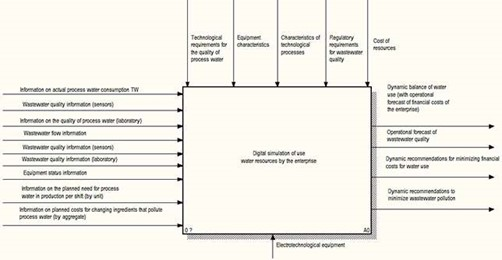
\includegraphics[width=15cm]{фигура1.jpg}
   \caption{Context diagram for modeling water use of a milk processing plant}
   \label{Fig. 1}
\end{figure}

\begin{figure}[H]
    \centering
    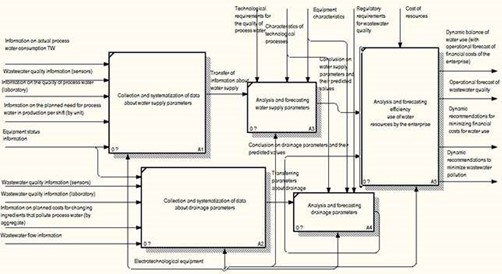
\includegraphics[width=15cm]{фигура2.jpg}
    \caption{First level of context diagram decomposition}
     \label{Fig. 2}
\end{figure}

\begin{multicols}{2}
\fontsize{10}{13}\selectfont
    based on benchmarking and expert opinions.\par Main planned products:
    \begin{itemize}[leftmargin=7mm]

    \item software (SP), which can be used by all enterprises,
including holding companies;
\item\nohyphens{ educational and methodological materials for continuous improvement of qualifications and retraining of
specialists in the field of digital technologies using
the created product.}
    \end{itemize}
    \nohyphens {At the same time, it should be noted that water use
processes, including the functioning of local treatment
facilities, are characterized by nonlinearity, nonstationarity, multifactorial, multiprocess nature, constant changes
in the structure of internal relationships, the presence of
significant hidden mutual influences between technological parameters, the use of separately functioning ones
when solving a single industrial problems of information
systems (for example, 5-6 industrial SCADA) [4]–[9].\vskip 0.2cm
Accordingly, the proposed (reasonable) transformation
(“intelligent decision support system – automated process
control system for water use — digital MES (MIS,
LIMS, EMI) resources — ERP”) requires a specialized
methodological apparatus of a new generation. \vskip 0.2cm
Such solutions include OSTIS Technology [10]. New
generation intelligent computer systems developed on its
basis are called OSTIS systems. The OSTIS Technology
is based on a universal method of semantic representation
(coding) of information in the memory of intelligent
computer systems, called the SC code. SC code texts
(sc-texts, sc-constructions) are unified semantic networks
with a basic set-theoretic interpretation. Elements of}
\end{multicols}
\newpage

\end{document}